\subsection{Background}
\subsubsection{Image processing}
An image can be seen as a mathematical function $i(x,y)$ where $x$ and $y$ are the spatial coordinates and the output is a color at position $(x,y)$. If the color has a discrete quantities and the total image has a finite element of samples, it is called a \emph{Digital Image}. The samples each has a unique spatial coordinate and are referred to as \emph{pixels}. The field of \emph{Digital Image Processing} refers to processing a digital image and its pixels. Every time Image Processing is mentioned in this theis, it is assumed that it refers to Digital Image Processing. 
\newline

The most typical application in image processing is when an algorithm is used to create a modified output image from an input image. This can be operations such as blur, sharpen and noise removal, all common techniques in standard image editing software. Figure \ref{lena} shows and example of a blur operation.
\begin{figure}[ht!]
\centering

\includegraphics[width=80mm]{img/klas.png}
\caption{A blur algorithm is applied on an input image and produces a blurred output image.}
\label{lena}
\end{figure}

Another possible application would be where a function is used on an input image to extract information and features in the image. Figure \ref{feature} shows an example of a feature detection algorithm performed on an image containing a face. The algorithm manages to locate features such as nose, mouth and the eyes. Although the image is processed, not everyone agrees that this is typical application of image processing. Some people think this belong to the computer vision field. 

\begin{figure}[ht!]
\centering
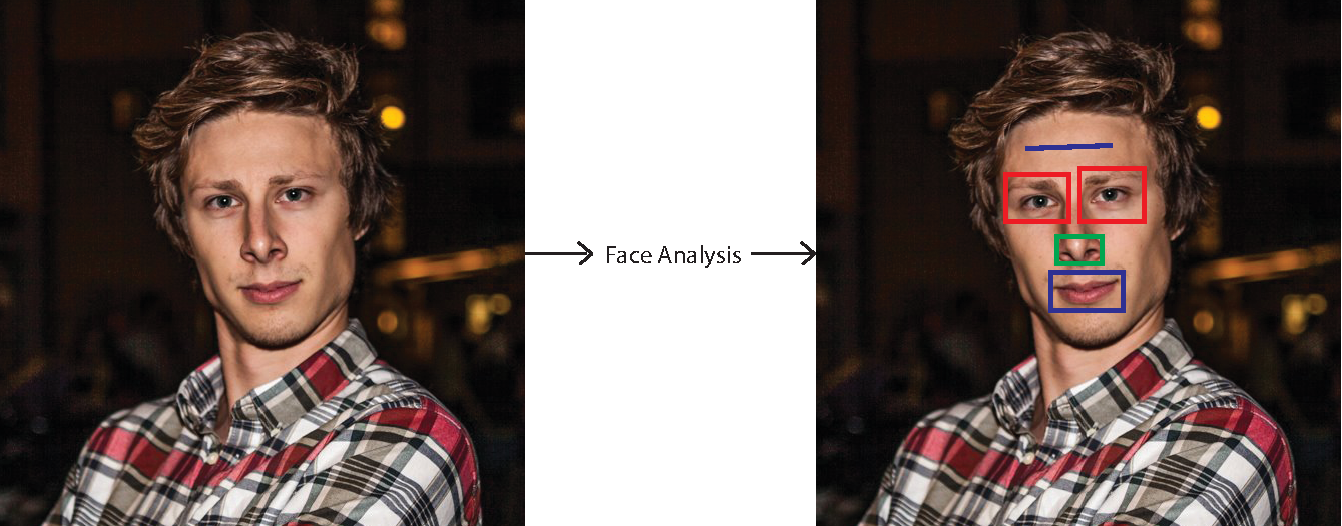
\includegraphics[width=80mm]{img/feature.pdf}
\caption{The input image of a face is analyzed to find features such as nose, mouth and eyes.}
\label{feature}
\end{figure}

\subsubsection{The evolution of computing hardware}

In the early 1960s, computers finally had enough computing power to perform meaningful image processing. The \emph{Jet Propulsion Laboratory} processed images of the moon captured by the on-board camera on the space probe \emph{Ranger 7} where they corrected image disortion. Later on, fields such as medical imaging astronomy started exploring the field of image processing. 
\newline

As the years passed by, the capacity of the computing hardware found in computers would keep improving. The term \emph{Moore's Law} was introduced based on a statement from the co-founder of Intel Corporation saying that the transistor count in integrated circuits are increasing by a factor of two every year. This was one of the reasons why the computing capability of processors kept increasing. The faster a processor's clock is operated, the faster a floating point computation is. In the early 1980s, the CPUs ran with internal clocks operating around 1 MHz. Today, around 30 years later, most CPUs have clock speeds around 2-4 GHz, which is a whole magnitude faster. Figure \ref{intelcpu} gives an overview of the transistor count and clock speeds of Intel CPUS the last 40 years.
\newline
\begin{figure}[ht!]
\centering
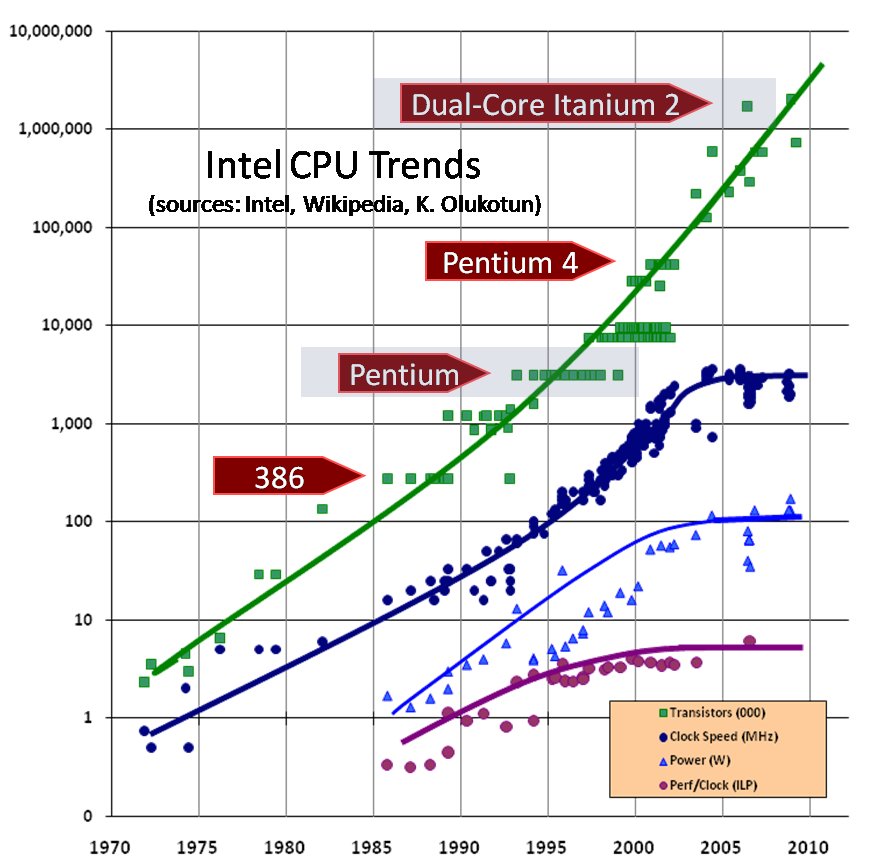
\includegraphics[width=70mm]{img/CPU.png}
\caption{The CPU transistor count has been growing exponentionally in the last 40 years.}
\label{intelcpu}
\end{figure}

Due to power and heat restrictions and the physical size of the current transistors, it is hard to keep improving the clock speeds. As of recent, the focus has shifted towards parallel computing and multicore processing units.

\subsubsection{GPU computing}

Computer games started became more popular in the 1990s. Computing was the big bottleneck in 3D graphics and it was hard to produce good real-time solutions. Therefore, companies started to experiment with a new computing device, the \emph{Graphical Processor Unit}, GPU. Instead of doing everything on the CPU, lighting computations and transforms of 3D coordinates could now entirely be done on the GPU. Since the computations of each pixels could be calculated independently of the others, it motivated the use of parallelism. 

\begin{figure}[ht!]
\centering
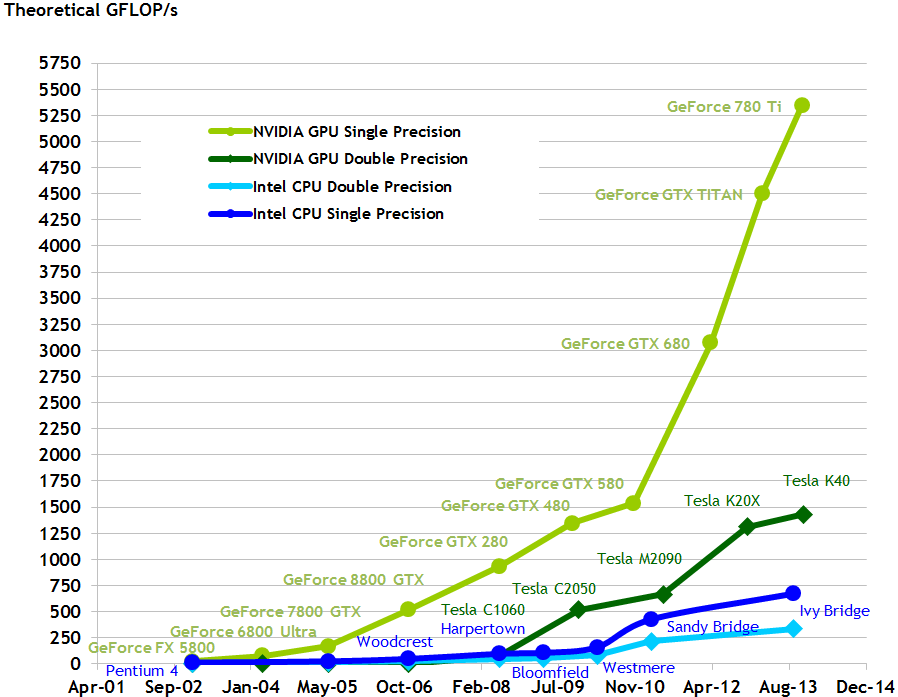
\includegraphics[width=90mm]{img/flops.png}
\caption{A comparison of theoretical floating point operations per second between CPUs and GPUs.}
\label{flops}
\end{figure}

When a GPU uses its full power and all computing units are used to maximum efficiency, a GPU is a lot faster than a CPU in terms of floating point operations per second. Figure \ref{flops} shows a comparison between the most recent CPUs and GPUs. The reason why the GPU is has lot higher theoretical maximu is because it is specalized for compute-intensive and highly parallel computations. It is therefore designed in a way that more transistors are devoted for data processing rather than data caching and flow control (which a CPU handles a lot better). 
